% Results Part One: Adsorption energy prediction from eDOS with CNN

\section{Results}

\subsection{Adsorption energy prediction from electronic density of states with convolutional neural network}

% Figure 2: CNN for eDOS
\begin{figure}[htbp]
    \centering
    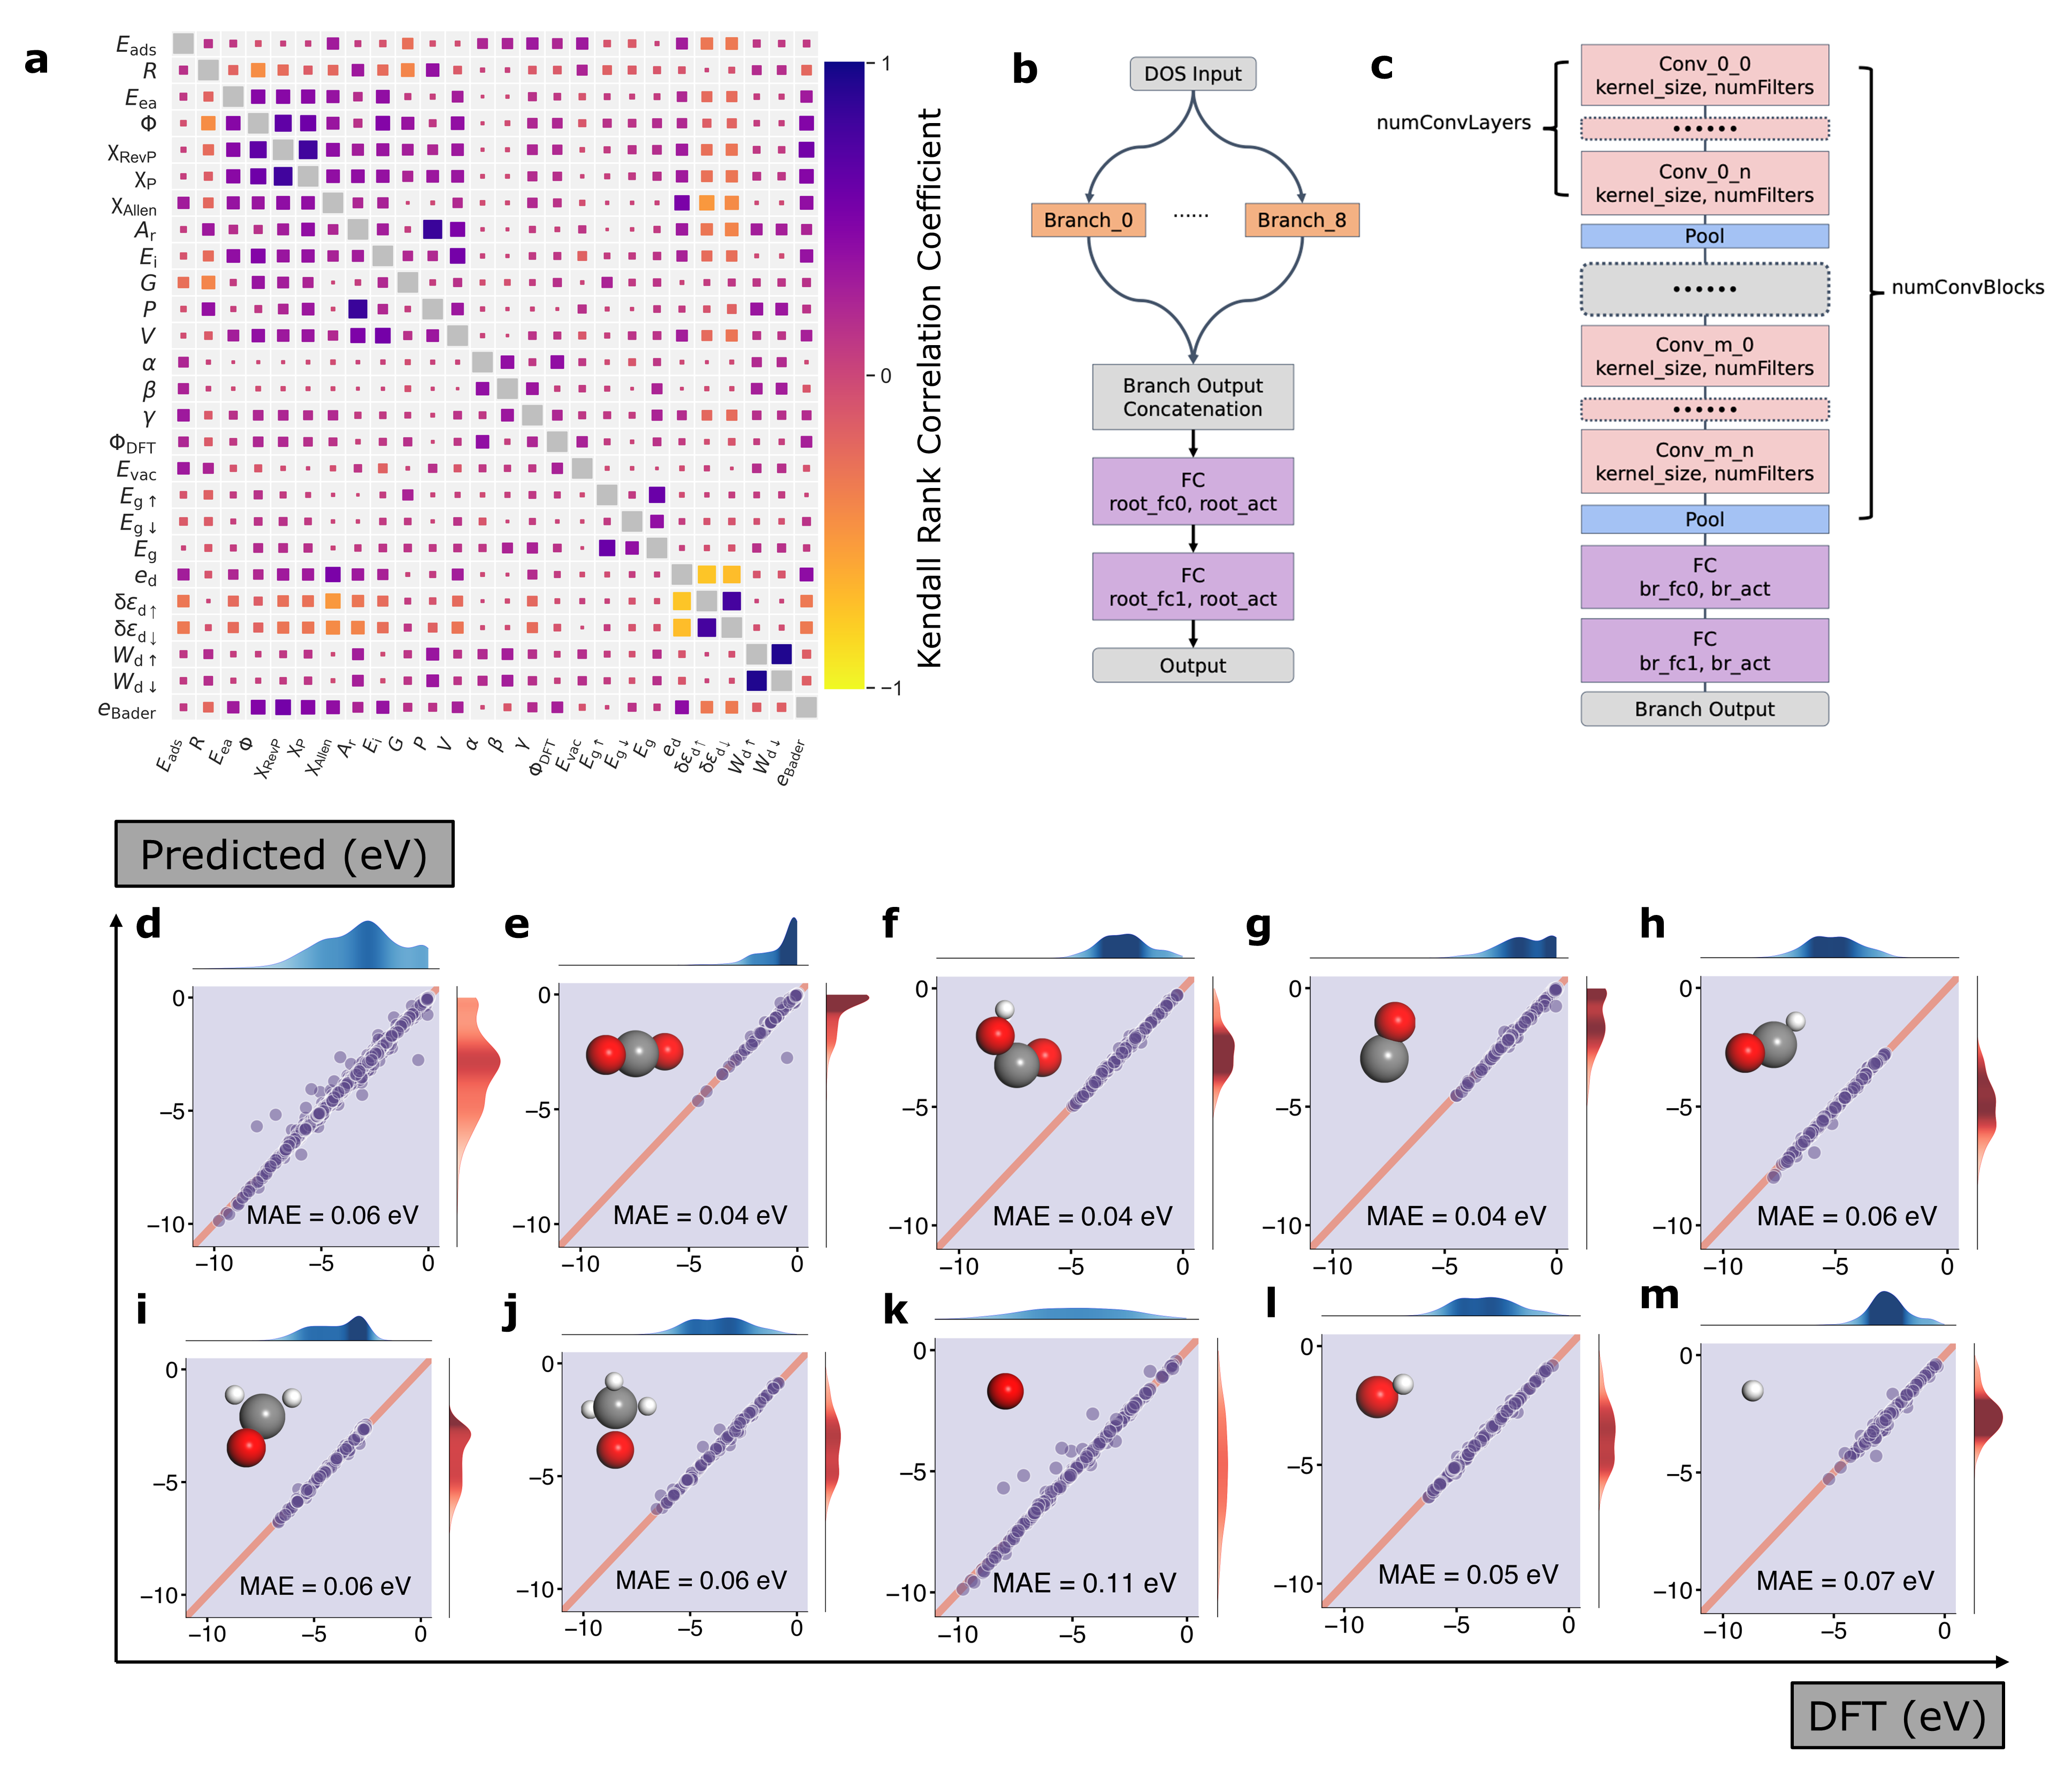
\includegraphics[width=\textwidth]{main_fig2_cnn.png}
    \caption{\textbf{CNN for Electronic Density of States.}
    \textbf{a}. Kendall rank correlation map illustrating the correlation
    between adsorption energy and some electronic and elementary descriptors.
    Definitions of the notations are provided in
    Supplementary \cref{supp_table15:descriptor_notations}.
    \textbf{b}-\textbf{c}. Architectural of (\textbf{b})the root and
    (\textbf{c})each branch of the CNN model.
    The architecture remains consistent across individual branches.
    \textbf{d}-\textbf{m}. Parity plots demonstrating the performance of the
    CNN model across nine adsorbates:
    (\textbf{d}) all adsorbates, (\textbf{e}) CO\textsubscript{2}, (\textbf{f})COOH,
    (\textbf{g})CO, (\textbf{h})CHO, (\textbf{i}) CH\textsubscript{2}O,
    (\textbf{j}) OCH\textsubscript{3}, (\textbf{k})O, (\textbf{l})OH, and (\textbf{m})H.
    The augmentation data are not displayed in the plots nor included in MAE evaluations.
    Kernel density estimate results are shown along the top and right sides of the main plot,
    representing DFT calculations and CNN model prediction distributions, respectively.}
    \label{main_fig2:cnn_for_eads}
\end{figure}

Originating from the pioneering work of Hammer and Nørskov \cite{hammer2000theoretical},
the d-band center model has emerged as a successful paradigm for employing descriptor to understand and predict the adsorption behavior on transition metal surfaces.
To investigate alternative electronic and elementary descriptors that may serve as more suitable substitutes for the d-band center model in the context of SACs,
we performed Kendall rank correlation analysis to account for both linearity and non-linearity \cite{kendall1938new}.
The correlation coefficient map, as presented in \cref{main_fig2:cnn_for_eads}a, highlighted the d-band center as the most informative descriptor with a Kendall's $\tau$ coefficient of -0.33, and followed by the vacuum level and electronegativity.
However, d-band center alone does not suffice for accurate predictions of intermediate adsorption energy as illustrated in the scatter plot Supplementary \cref{supp_fig18:dband_vs_eads}, and therefore, refinements are imperative.
Unlike bulk transition metal surfaces, where the variations in the d-band centre account for the majority of the adsorption energy variations \cite{norskov2011density, takigawa2016machine}, the unique structure of SACs introduces more variables rather than d-band center that are intrinsically correlated with the variations of adsorption energy.
This finding also interpreted that in some reported prior studies, indicating that depending solely on the d-band center may be insufficient for accurate adsorption energy predictions in the context of SACs \cite{sun2022going, fung2020descriptors, di2022universal, yuan2020descriptor, huang2020rational}.
As a result, the development of a method tailored specifically for catalysts like SACs becomes essential.

In our study, we employ CNN, a renowned deep learning method proficient in capturing spatial hierarchy from matrix-like data, such as the eDOS.
Notably, CNN's autonomy from prior knowledge and human intervention during feature extraction renders it more efficient than traditional machine-learning methods.
Our approach harnesses the entire 2D eDOS with a multi-branch CNN model.
\cref{main_fig2:cnn_for_eads}b and \cref{main_fig2:cnn_for_eads}c delineate the model and its branches.
The workflow involves processing the entire 2D eDOS as input, segregating orbitals into branches, and directing the concatenated outputs through another convolutional block, which generates the adsorption energy prediction.
Sharing learnable parameters across branches optimizes computational efficiency.
By leveraging the CNN model, we predicted adsorption energies from the eDOS of supported single atoms, and validated through parity plots (\cref{main_fig2:cnn_for_eads}d-m).
The model predicts adsorption energies across nine species within the CO\textsubscript{2}RR process and competing HER side reaction, attaining an averaged MAE of 0.06 eV.
This MAE aligns with the established precision of DFT methods, which typically range between 0.1-0.2 eV concerning experimental measurement \cite{wellendorff2015benchmark, kirklin2015open, lejaeghere2016reproducibility}.
The full list of prediction errors is available in Supplementary \cref{supp_table18:cnn_mae}.
These results confirm the CNN model's ability to predict adsorption energies from eDOS input.
Moreover, they suggest the potential for predicting adsorption energies for SACs using eDOS, although this would demand more sophisticated feature engineering techniques.

In terms of adsorption energy prediction, the CNN model maintained consistency across diverse elemental compositions and varied adsorption strengths.
It handled species containing oxygen, hydrogen, and carbon atoms equally well, spanning an adsorption energy range from 0 to 10 eV.
Significantly, after training the CNN model, making predictions (inferences) scales only linearly with system size and demands considerably less computational resources compared to DFT calculations \cite{chandrasekaran2019solving}.
Conversely, unlike QM based methods, which could generate reasonably precise energy estimation for individual candidates, CNN relies on extensive datasets to ensure reliable predictions.
In our case, the original dataset comprised 2052 samples, leading to a CNN model with a validation MAE of 0.3725 eV.
In pursuit of enhanced prediction accuracy, we proposed a data augmentation method detailed in the Methods section.
This augmentation resulted in an expanded dataset of 12312 samples, enhancing prediction performance with a reduced validation MAE of 0.1736 eV.
Comparatively, our CNN model diverges from prior attempts, notably Fung's pioneer work \cite{fung2021machine}, by requiring only the eDOS of supported single metal atom alone and adsorbate.
This revision eliminated the necessity for a complete set of substrate and adsorbate eDOS and significantly reduced computational cost.
We foresee the potential in the applicability of our method to diverse species and electrocatalytic reactions, given the availability of comprehensive datasets.
The strength of our CNN model lies in its freedom from element- or adsorbate-specific parameters, relying solely on eDOS as input.
This adaptability opens up the possibility for its utilization in a wide array of electrocatalytic studies.
